\documentclass{beamer}
\mode<presentation>
{
  \usepackage{theme/theme}
  \setbeamercovered{transparent}
}

\usepackage{amsmath,amssymb,amsfonts}
\usepackage{times}
\usepackage{graphicx}
\usepackage{fancyvrb}
\usepackage{array}
\usepackage{colortbl}
\usepackage{tabularx}
\usepackage{fontspec}
\usepackage{minted}
\usepackage{libs/tikz-uml}

% Uncomment me when you need to insert code
\usepackage{color}
\usepackage{listings}
% End Code

% Uncomment me when you need video or sound
\usepackage{multimedia}
\usepackage{hyperref}
% End video

% End Header

% Titlepage
\title{L1. Laboratory Introduction}
\author{Enterprise Software Architectures}
\institute
{
  Bachelor's Degree in Computer Engineering
}
\date{Academic course 2025/26}
% End Titlepage

\AtBeginSection[]{
  \begin{frame}
    \centering
    \begin{beamercolorbox}[sep=8pt,center]{title}
      \usebeamerfont{title}\insertsectionhead
    \end{beamercolorbox}
  \end{frame}
}

% Slides
\begin{document}

\begin{frame}
  \titlepage
\end{frame}

\begin{frame}
  \frametitle{L1. Laboratory Introduction}
  \tableofcontents[subsectionstyle=show]
\end{frame}

\section{Block A - Introduction to Enterprise Software}
\begin{frame}
  \frametitle{Quick history lesson}

  \begin{columns}[T,onlytextwidth]
    \column{0.5\textwidth}
    \centering
    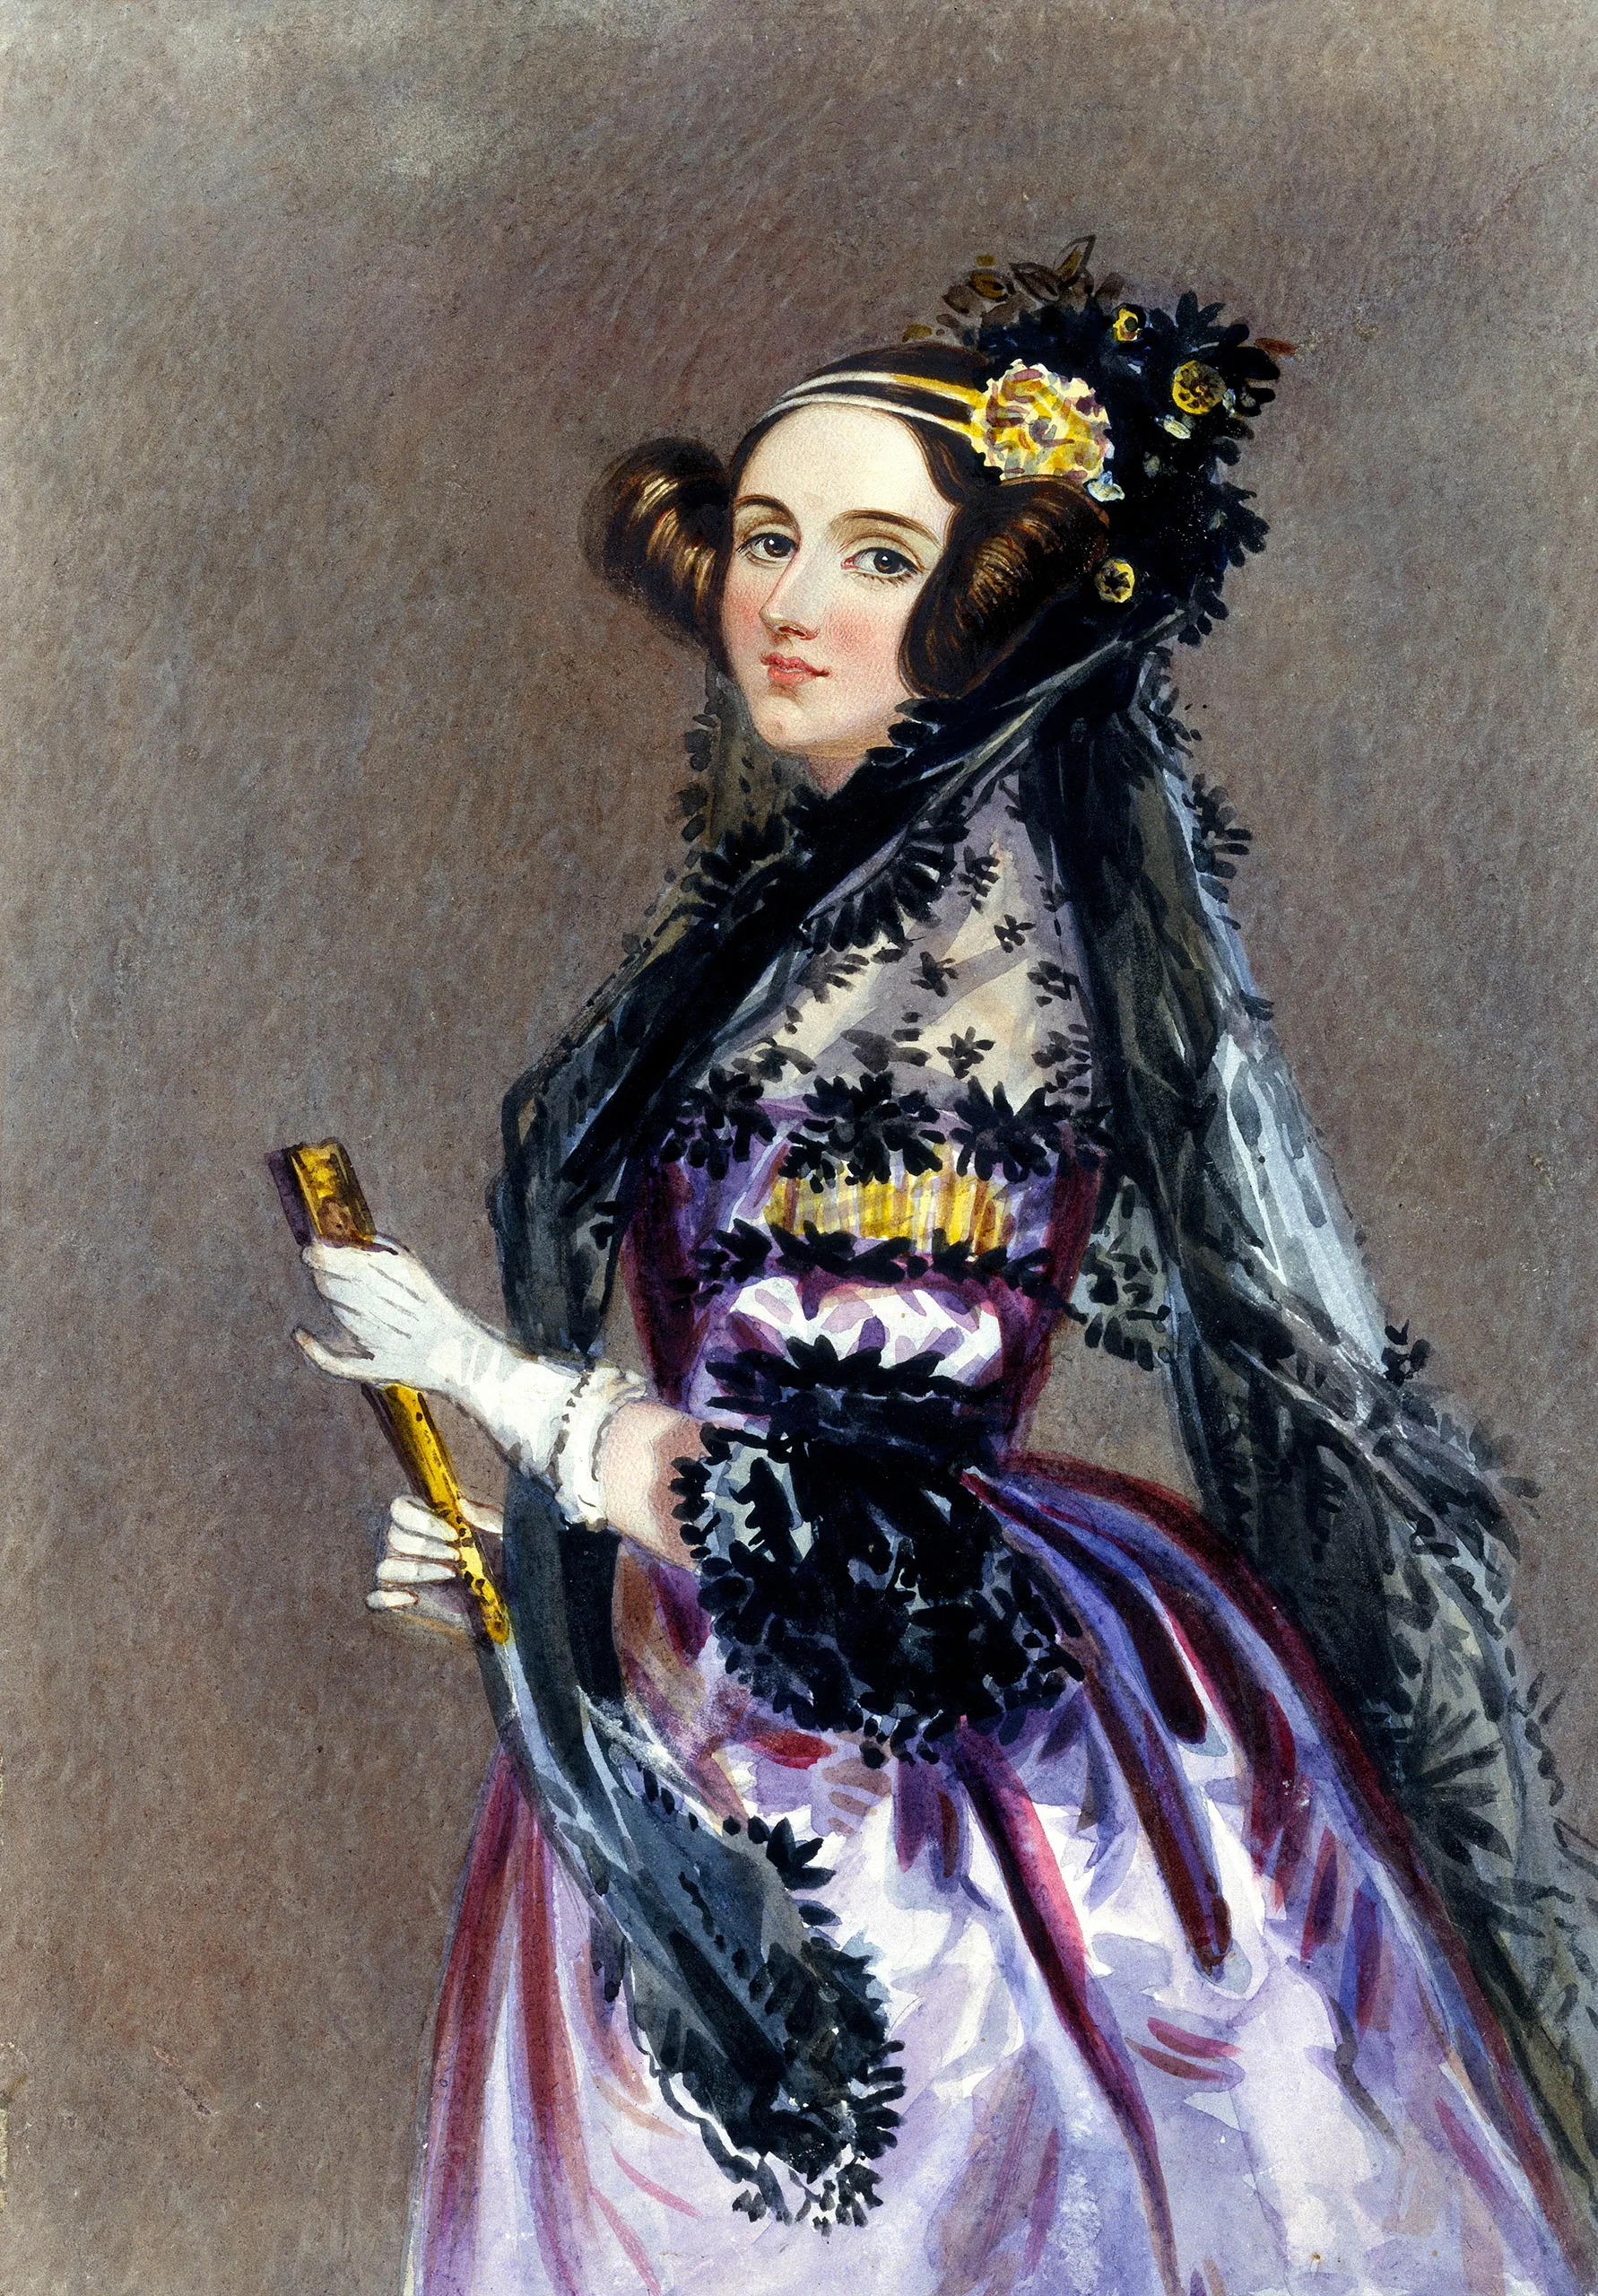
\includegraphics[height=0.7\textheight]{images/lovelace.png}

    \visible<2->{\vspace{0.5ex}\scriptsize Ada Lovelace (first programmer)}
    \column{0.5\textwidth}
    \centering
    \includegraphics[height=0.7\textheight]{images/hamilton.jpg}

    \visible<2->{\vspace{0.5ex}\scriptsize Margaret Hamilton (first software engineer)}
  \end{columns}
\end{frame}

\begin{frame}
  \frametitle{What is Enterprise Software?}

  \begin{itemize}
    \item \textbf{Lovalace} wrote the first algorithms for Babbage's Analytical Engine. They were \textbf{simple programs} and were meant as an intellectual exercise or proof of concept.

      \vfill

    \item \textbf{Hamilton} and her \textbf{MIT team} developed the on-board flight software for NASA's Apollo Guidance Computer. It was the \textbf{most complex} and \textbf{safest} software ever written at the time.
  \end{itemize}

\end{frame}

\begin{frame}
  \frametitle{What is Enterprise Software?}

  You are not Ada Lovelace, you are Margaret Hamilton.
  \vfill
  \begin{itemize}
    \item Software Engineers work in \textbf{teams} to solve \textbf{complex problems} with \textbf{real stakes} (potentially human lives).
    \item Complex software problems require different \textbf{architecture patterns} and \textbf{development strategies} compared to simple software.
  \end{itemize}

\end{frame}

\begin{frame}
  \frametitle{Software Engineers are Engineers}

  \begin{columns}[T,onlytextwidth]
    \column{0.7\textwidth}
    Engineers...
    \begin{itemize}
      \item Don't reinvent the wheel: use \textbf{standards} (IEEE, ISO...), \textbf{patterns} and \textbf{good practices}.
      \item Care about long-term \textbf{reliability} and \textbf{performance}.
      \item Work within \textbf{requirements} and \textbf{budgets}.
      \item Use \textbf{formal diagrams} to communicate.
      \item Build prototypes and run controlled experiments.
    \end{itemize}

    \column{0.3\textwidth}
    \centering
    \begin{tikzpicture}
      \umlclass{SoftwareEngineer}{}{}
      \umlclass[x=0,y=2]{Engineer}{}{}

      \umlinherit[geometry=-|]{SoftwareEngineer}{Engineer}
    \end{tikzpicture}

  \end{columns}

\end{frame}

\section{Block B - Project overview}
\subsection{Basic requirements}
\begin{frame}
  \frametitle{Basic requirements}
  \begin{itemize}
    \item The client wants the frontend to be a web-app.
      \begin{itemize}
        \item This is good for us. We can write one web-app instead of creating native applications for Windows, Android, iOS, etc.
      \end{itemize}
    \item We need to persist information about the users, teams, etc.
      \begin{itemize}
        \item We'll need a database.
      \end{itemize}
    \item The entire system must be performant, reliable and secure.
  \end{itemize}
\end{frame}

\subsection{Physical architecture}
\begin{frame}
  \frametitle{Physical architecture}
  We'll use a simple and battle-tested Client-Server architecture:
  \begin{figure}
    \includegraphics[scale=1]{images/diagrams/PhysicalArch1.pdf}
    \caption{Physical architecture high-level overview}
  \end{figure}
\end{frame}

\begin{frame}
  \frametitle{Choosing technologies}

  We'll pick the most widely used technologies for each area:
  \url{https://survey.stackoverflow.co/2025/technology/}
  \newline
  \newline
  Other decisions that need to be made:
  \begin{itemize}
    \item Client-Side Rendering vs Server-Side Rendering
    \item REST vs GraphQL
      \begin{itemize}
        \item \url{https://blog.postman.com/graphql-vs-rest/}
      \end{itemize}
  \end{itemize}
\end{frame}

\begin{frame}
  \frametitle{Physical architecture \& Used technologies}
  \begin{figure}
    \includegraphics[scale=1]{images/diagrams/PhysicalArch2.pdf}
    \caption{Physical architecture high-level overview}
  \end{figure}
\end{frame}

\section{Block C - Introduction to REST}

\subsection{What is REST?}
\begin{frame}
  \frametitle{What is REST?}
  \begin{block}{Problem}
    We need to define an interface between our frontend (web-app running in client devices) and our backend (Java program running in the server).
  \end{block}

  REST (Representational State Transfer) is an architectural pattern where we map each \textbf{backend resource} to a \textbf{URI}.
  \newline
  When the client wants to read or modify information, it performs an HTTP request to the corresponding endpoint.

\end{frame}

\subsection{RESTful API design}
\begin{frame}
  \frametitle{RESTful API design: Steps}

  \begin{enumerate}
      \only<1>{
      \item Identify which \textbf{resources} should be exposed to the frontend. \newline \textit{Tip:} They usually match the most important classes in your ER model.
      }
      \only<2>{
        \setcounter{enumi}{1}
      \item Find a good URI for each resource. URIs should read like a filesystem path, with alternating {\color{blue!60!black}collections} and {\color{green!50!black}elements}.
      }
      \only<3>{
        \setcounter{enumi}{2}
      \item See which \textbf{HTTP metods} make sense for each URI. \newline We will use a simplified version of REST with only 4 verbs:
      }
  \end{enumerate}

  \vfill

  \only<1>{
    \centering
    \begin{tikzpicture}
      \umlclass{User}{...}{}
      \umlclass[x=6,y=0]{Book}{...}{}

      \umlassoc[geometry=-|-, mult1=*, mult2=*, pos2=2.8, name=assoc]{User}{Book}
      \umlassocclass[x=3,y=-1.5]{FavoriteBook}{assoc-2}{...}{}
    \end{tikzpicture}
  }
  \only<2>{
    \centering
    \begin{tabular}{@{}l l@{}}
      \textbf{URI} & \textbf{Meaning} \\
      \hline
      \texttt{/{\color{blue!60!black}books}} & Collection of all books \\
      \texttt{/{\color{blue!60!black}books}/{\color{green!50!black}187}} & Book with ID = 187 \\
      \texttt{/{\color{blue!60!black}users}} & Collection of all users \\
      \texttt{/{\color{blue!60!black}users}/{\color{green!50!black}mike}} & User with username = "mike" \\
      \texttt{/{\color{blue!60!black}users}/{\color{green!50!black}mike}/{\color{blue!60!black}favoriteBooks}} & List of Mike's favorite books \\
      \texttt{/{\color{blue!60!black}users}/{\color{green!50!black}mike}/{\color{blue!60!black}favoriteBooks}/{\color{green!50!black}187}} & FavoriteBook association \\
    \end{tabular}
  }
  \only<3>{
    \begin{itemize}
      \item {\color{green!60!black}\texttt{GET}}: Read an \textbf{entity}, or list all members of a \textbf{collection}. \newline The GET method is always \textit{safe}, it never modifies data.
      \item {\color{orange!80!black}\texttt{POST}}: Create a new entity in a \textbf{collection}.
      \item {\color{blue}\texttt{PUT}}: Modify/update an \textbf{entity}.
      \item {\color{red}\texttt{DELETE}}: Delete an \textbf{entity}.
    \end{itemize}

    \begin{exampleblock}{Important}
      Notice that \texttt{GET} is the only verb that can be used with both collection and entity URIs. \newline Some APIs allow using \texttt{DELETE} on an entire collection, but that is considered dangerous and a bad practice.
    \end{exampleblock}
  }

\end{frame}

\begin{frame}
  \frametitle{RESTful API design: Examples}

  List/search books. Filters are sent via \textbf{query parameters}:\newline
  \texttt{{\color{green!60!black}GET} /books\textbf{?year=2017\&title=Origin}}
  \newline

  Create a new book. Data is sent via \textbf{HTTP request body}:\newline
  \texttt{{\color{orange!80!black}POST} /books}\newline
  \texttt{\{"title": "The Hobbit", "year": "1937", ...\}}
  \newline

  Update user info. Only \textit{modified} fields are sent via \textbf{body}:\newline
  \texttt{{\color{blue}PUT} /users/mike}\newline
  \texttt{\{{"birthday": "2003-04-19"}\}}
  \newline

  Un-favorite a book:\newline
  \texttt{{\color{red}DELETE} /users/mike/favoriteBooks/187}\newline
\end{frame}

\begin{frame}
  \frametitle{RESTful API design: Additional considerations}

  \begin{itemize}
    \item The request body is always a \textbf{JSON object}, and can only be used in \texttt{PUT} and \texttt{POST} (never in \texttt{GET} or \texttt{DELETE}).
    \item The response body is always a \textbf{JSON object or array}.
    \item The HTTP response code can be either:
      \begin{itemize}
        \item \textbf{\color{green!60!black}\texttt{200 OK}} for \texttt{GET}, \texttt{PUT} and \texttt{DELETE}. \textbf{\color{green!60!black}\texttt{201 CREATED}} for \texttt{POST}.
        \item \textbf{\color{orange!80!black}\texttt{4xx}} for client errors (incorrect API usage).
        \item \textbf{\color{red}\texttt{5xx}} for server errors (unhandled errors in the backend).
      \end{itemize}
    \item Not all users can perform all operations! The client must send an \texttt{Authorization} header which the backend validates.
  \end{itemize}
\end{frame}

\begin{frame}
  \frametitle{RESTful API design: Additional considerations}

  \begin{block}{Problem}
    What if I need to add a functionality that doesn't map well to any resource URI? For example: "Resend the user's verification mail"
  \end{block}

  In this case, we create a new URI corresponding to a \textbf{verb} (action) instead of a \textbf{noun} (resource).\newline
  \texttt{{\color{orange!80!black}POST} /users/mike/\textbf{resendVerificationMail}}\newline

  \begin{itemize}
    \item Use \texttt{{\color{orange!80!black}POST}} for non-idempotent actions (such as sending notifications) and \texttt{{\color{blue}PUT}} for idempotent actions (such as subscribing to a topic).
  \end{itemize}

\end{frame}

\section{Work assignment}
\begin{frame}
  \frametitle{Work assignment}

  \begin{enumerate}
    \item Make sure you have completed the "Group creation" test. Wait to get access to the "UdL-EPS-SoftArch-Igualada" GitHub organization.
    \item Clone the backend (Java) repository. Be careful \textbf{not} to clone the \textit{template} repo.
    \item Create and push new branch for your changes. You \textbf{do not} need to create a \textit{fork} of the repository.
    \item Write the basic code for the domain model classes that were assigned to you in class. You \textbf{must} use \href{https://en.wikipedia.org/wiki/Pair_programming}{pair programming}. Use the existing model classes as examples.
    \item Commit your changes with a descriptive message, and create a Pull Request.
  \end{enumerate}
\end{frame}

\end{document}
